It has been over half a century since renowned astrophysicist Sjur
Refsdal first hypothesized the use of a supernova (SN) resolved into
multiple images as a cosmological tool. In recent years, the first
multiply-imaged core-collapse (CC) SN Refsdal \citep{Kelly:2015a}, and
subsequently the first Type Ia SN iPTF16geu \citep{Goobar:2016}, have
been discovered (Figure 1A-C). As the light for each of the multiple
images follows a different path through the expanding universe and
through the lensing potential, the SN images appear delayed by hours
(for galaxy-scale lenses) or years (for cluster-scale lenses). The
next decade is expected to yield observations of tens to hundreds of
multiply-imaged SNe \citep{Oguri:2010a}, yet there is no public
software package for analyzing multiply-imaged SNe.

\begin{wrapfigure}{r}{.5\textwidth}
\centering
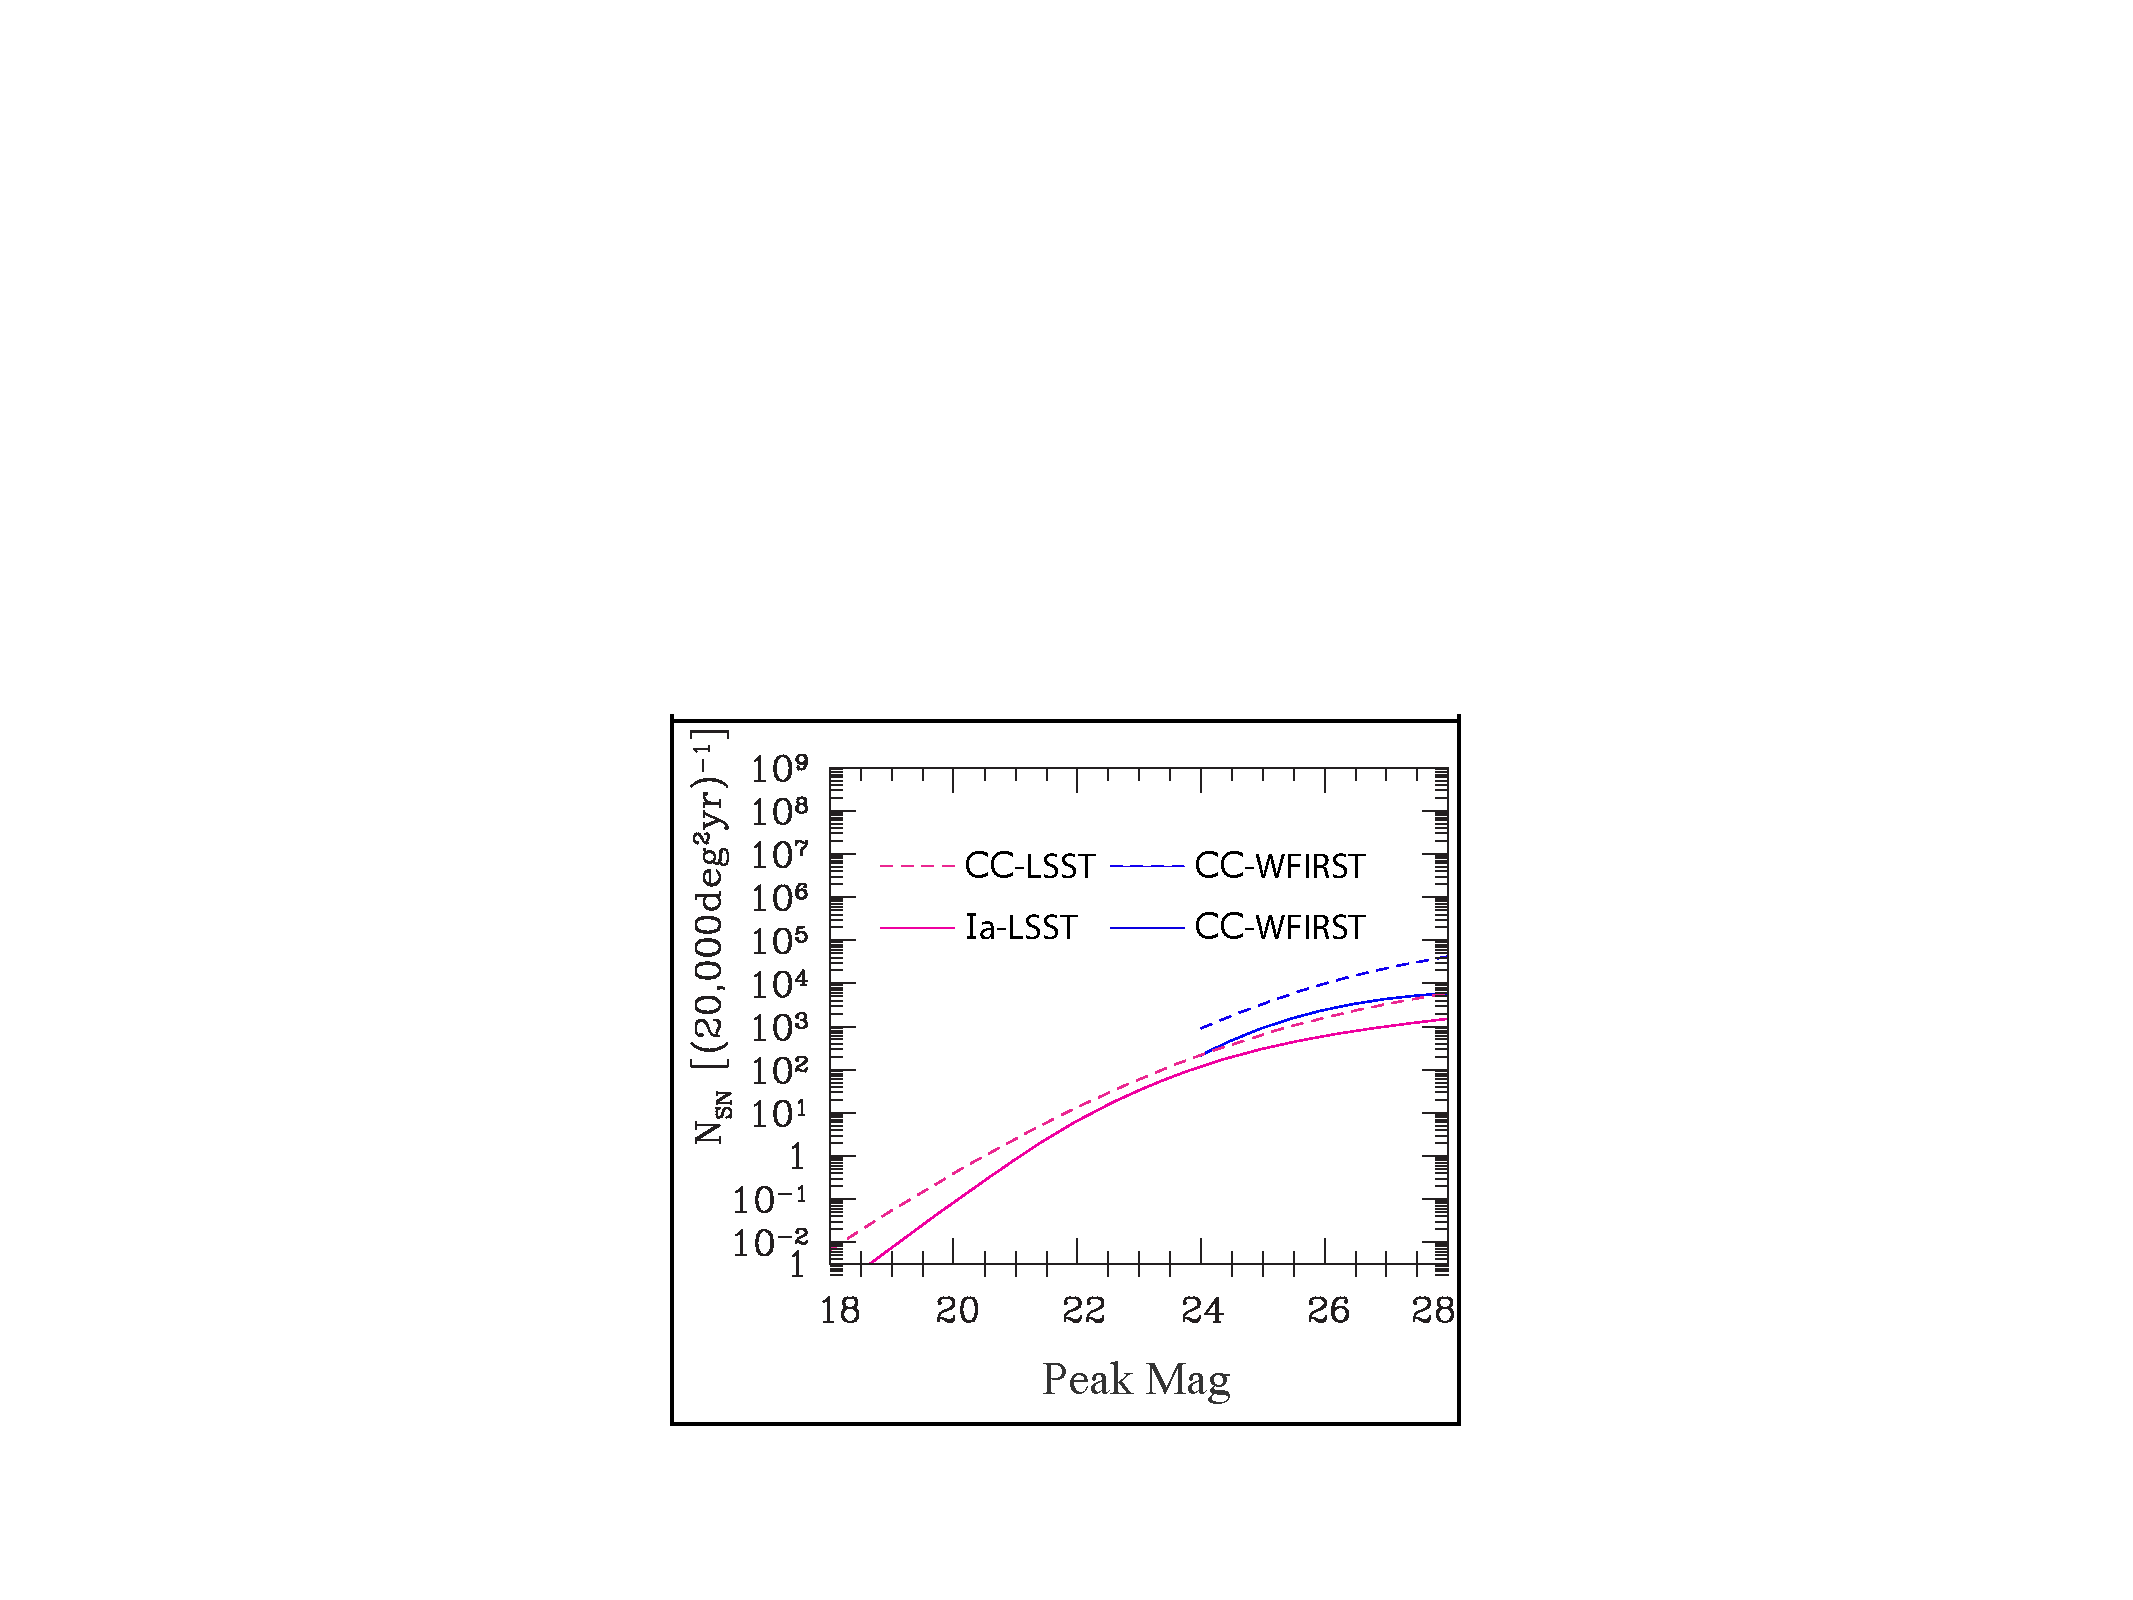
\includegraphics[height=.4\textwidth]{FIG/wfirst_lsst}
\caption{
\noindent\fontsize{10}{14}\selectfont
Expected numbers of lensed SNe Ia and Core Collapse SNe for LSST
$(i_{peak,lim})$ and WFIRST $(H_{peak,lim})$ after one year of
observations. With this huge volume of lensed CC and Ia SNe
observations expected in the next decade, the open-source SNTD package
will be widely used and essential for analyzing this large WFIRST/LSST SN sample
(adapted from Oguri $\&$ Marshall 2010 \cite{Oguri:2010a}).}
\end{wrapfigure}

\noindent\underline{\textit{Intellectual Merit}} :
As the PI on an ongoing HST Archival Research Grant, \textbf{I am
developing the first open-source software package} in Python
(\textit{Supernova Time Delays} [SNTD]) that will enable a user to
precisely measure lens properties and time delays for the hundreds of
multiply-imaged SNe expected in the LSST/WFIRST era (Figure 1D). I
will use SNTD to make more precise time delay measurements for the two
currently documented multiply-imaged SNe. Properties of dark energy
and dark matter are still poorly understood and inadequately
constrained, but accurate measurements of the lensing magnification and
time delays for SN Refsdal can be used to test models for the dark
matter distribution in the lensing
object \cite{Rodney:2015a,Rodney:2016} or as a probe to test
cosmological models \cite{Suyu:2014}. As SN iPTF16geu is Type Ia,
providing more accurate time delay and luminosity distance
measurements will accomplish two critical goals. First, directly
measuring the source magnification will provide an important milestone
in breaking degeneracies in the lens
model \cite{Kolatt:1998,Oguri:2003b}. Second, precise determinations
of the time delays for a multiply-imaged Type Ia SN will provide a
measurement of the Hubble constant $H_0$ that is completely independent of the local
distance ladder, and the methodology and software I develop will
be \textbf{essential to future SN surveys} for tightening those
constraints.

Observations either by way of gravitational lensing, or by the next
generation telescope JWST, will provide a sample of extremely high
redshift SNe (Figure 2). Of interest in the early universe are
pair-instability (PI) and Population III (Pop III) SNe,
as \textbf{understanding these first stars is crucial to a wide range
of cosmology including the formation of primeval galaxies, initial
stages of cosmological reionization, and the origin of Supermassive
black holes} \cite{Whalen:2013}. Therefore, I will collect a sample
of high-z and gravitationally lensed SNe, and begin discerning
the properties of these poorly understood objects via powerful
lensing. With the SNe identified as weakly lensed, I will produce
careful magnification measurements and make small corrections
to the Hubble diagram. In addition to searching for PI and Pop III SNe
and studying their physical properties, I will include theoretical
light curve templates for both objects in SNTD, so that future
observations can be identified and both lens properties and progenitor
physics studied.

\begin{wrapfigure}{r}{.5\textwidth}
\centering
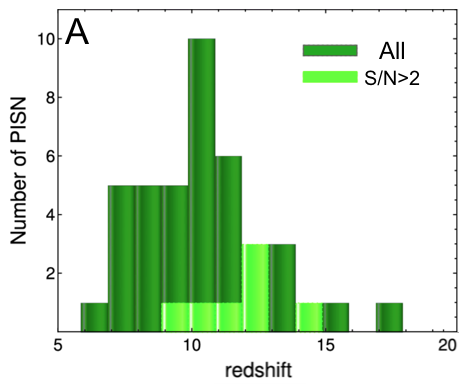
\includegraphics[height=.3\textwidth]{FIG/pisn_rates}
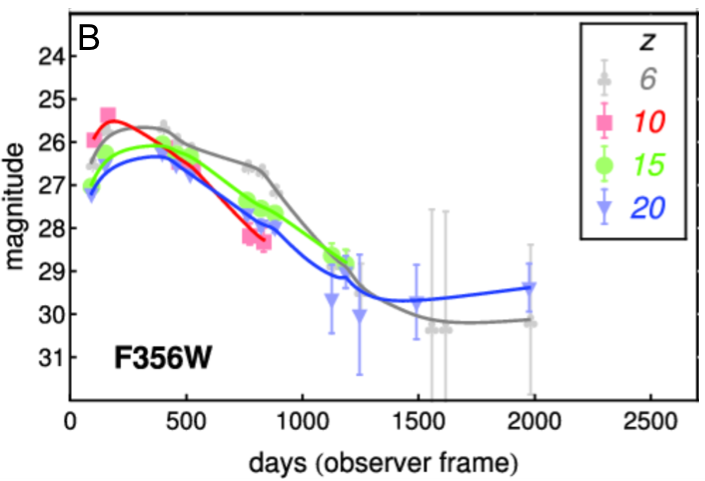
\includegraphics[height=.3\textwidth]{FIG/jwst_sim}
\caption{
\noindent\fontsize{10}{14}\selectfont
(A) Histogram showing the dozens of expected PISN observations as a
function of redshift for a single JWST survey realization, covering
0.06$\%$ of the sky over the course of 5 years. (B) Colored curves
depict simulated JWST NIRCam PISN observations in the F356W
filter. These light curves show that the PISNe will be visible for
thousands of days, making observations extremely likely in each field,
which makes their inclusion in SNTD essential to future work with JWST (Figures
adapted from Souza et al. 2013 \cite{Souza:2013}).}
\end{wrapfigure}

\noindent\underline{\textit{Research Summary}}:
First, I will complete the python software package SNTD, and write a
publication presenting its capabilities and validation. Next I will
perform the reanalysis of SN Refsdal and SN iPTF16geu using SNTD,
writing a second publication presenting the more precise time delay
measurements, detailing the methodology required for these analyses,
and obtaining a constraint on $H_0$ from iPTF16geu. Finally, I will
add theoretical light curves for PISN and POP III SNe to the SNTD
package, and obtain a gravitationally lensed SN sample to study the
physics of these first stars. With the weaker lensed objects, I will
perform Hubble diagram magnification adjustments. From this last
component of my research, I will complete two further publications:
one describing magnification corrections for Hubble diagram SNe and
their affect on $H_0$, and the other detailing the search for, and
ideally discovery of, PISNe and POP III SNe and their physical
properties. These \textbf{four publications} will be a clear measure of the
success of this work, and the software and methodologies developed
during the course of my research will be vital for future work
using the next generation of space telescopes.

\noindent\underline{\textit{Broader Impacts Summary}}:
Due to my academic experience at a young age, I am committed to
ensuring that no child's love of astronomy will go unfostered in my
community. It is crucial that childen who love STEM, and specifically
astronomy, are reinforced that this is a valid future career and that
a graduate degree is possible for them. Growing up in rural Maine,
graduate degrees were few and far between, and even the percentage of
high school graduates attending a 2-4 year college was only around
50$\%$. In my current community within Columbia, SC according to
City-Data.com, \textbf{only $27\%$ of people graduated from high
school, $13\%$ have a bachelor's degree, $3\%$ have a master's degree,
and $0\%$ have a PhD.} I will use my STEM outreach experiences with
NASA's ARSET program, as well as the techniques I learned volunteering
in elementary school math classrooms in college and tutoring high
school students while at Goddard, to help foster excitement for STEM
in my community. I have already discussed my plans with the local
after-school program leader, who was very excited to implement a
framework to encourage astronomy and STEM learning. By taking kids to
our local University observatory, and leading them through a series of
exciting and educational astronomical exercises throughout the year, I
hope to convince these students that \textbf{achieving higher degrees
is possible and valuable}, and break the viscious cycle of supressed
academic opportunities forming in my community.

\noindent\fontsize{10}{14}\selectfont
[1]Kelly, P. L., et al. 2015, Science, 347, 1123 [2]Goobar, A., et
al. 2016, arXiv:1611.00014v1 [3]Oguri, M., $\&$ Marshall, P. J. 2010,
MNRAS, 405, 2579 [4]Rodney, S. A., et al. 2015, ApJ, 811,70
[5]Rodney, S. A., et al. 2016, ApJ, 820, 50 [6]Suyu, S. H., et
al. 2014, ApJ, 788, L35 [7]Kolatt, T. S., $\&$ Bartelmann, M. 1998,
MNRAS, 296, 763 [8]Oguri, M., $\&$ Kawano, Y. 2003, MNRAS, 338, L25
[9]Whalen, D. J., et al. 2013, arXiv:1312.6330 [10]de Souza, R. S., et al. 2013, MNRAS, 436, 1555
\pagebreak

%measure of success:

%SNTD is open-source and so it'll be vetted and used by the entire community

%Growing sample of gravitationally lensed publically available where tools would be available (rubin & haden-''The discovery of a gravitationaly lensed supernova Ia at redshift 2.22)

%change gravitationally lensed sample -> strongly lensed

%Where are the strongly lensed ones coming from? HST revisiting frontier fields ``Buffalo'' -> Rodney is collaborator

%Figure out JWST Timeline (when will data be collected for GTO and ERS and cycle 1), more for high-redshift case not multiply-imaged. Highly magnified z>6 sne for GTO.

%Explicitly saying we have a small set of multiply imaged, tools important in the next decade

%First paragraph-->make it more of a thesis sentence at the end, instead of there is no current package. maybe also jwst high redshift sne for me to analyze.

%``Small chance from buffalo with hst and a much better chance with windhorst gto''. CLASH frontier, C-chains about 5. relics->about 3 more.

%take figure 1 text->moving it into main text. just make it either just the third figure or something describing the outcome of software package

%Figure 2-expected number of pair instability and POP III
